\subsection{Oversigt}\label{logical:oversigt}

Der er herunder opsat et pakkediagram over de delsystemer vi har indentificeret i projektet. Hver pakke symboliserer derved et system der skal implementeres individuelt. <<Flow>> fortæller at der er kommunikation imellem systemerne, og <<use>> symboliserer at systemerne benytter sig af pakken. Dybere forklaring af hvordan hver pakke er designet vil blive beskrevet i designdelen.

\begin{figure}[ht]
	\centering
    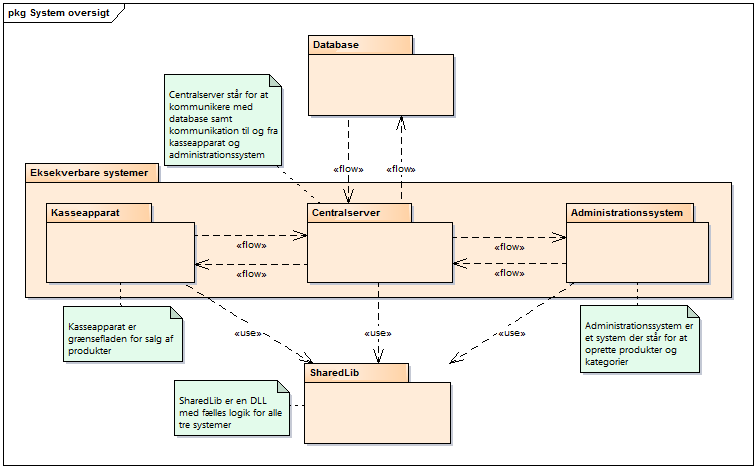
\includegraphics[scale=1]{Systemarkitektur/LogiskView/systemoversigt}
    \caption{Oversigt over systemet i pakker}
    \label{fig:system_oversigt}
\end{figure}

En nærmere beskrivelse af hver pakkes ansvar vil blive beskrevet på næste side under Arkitekturpakker.

\newpage

